% !TEX root = ../main.tex

\begin{figure}[t]
    \centering
    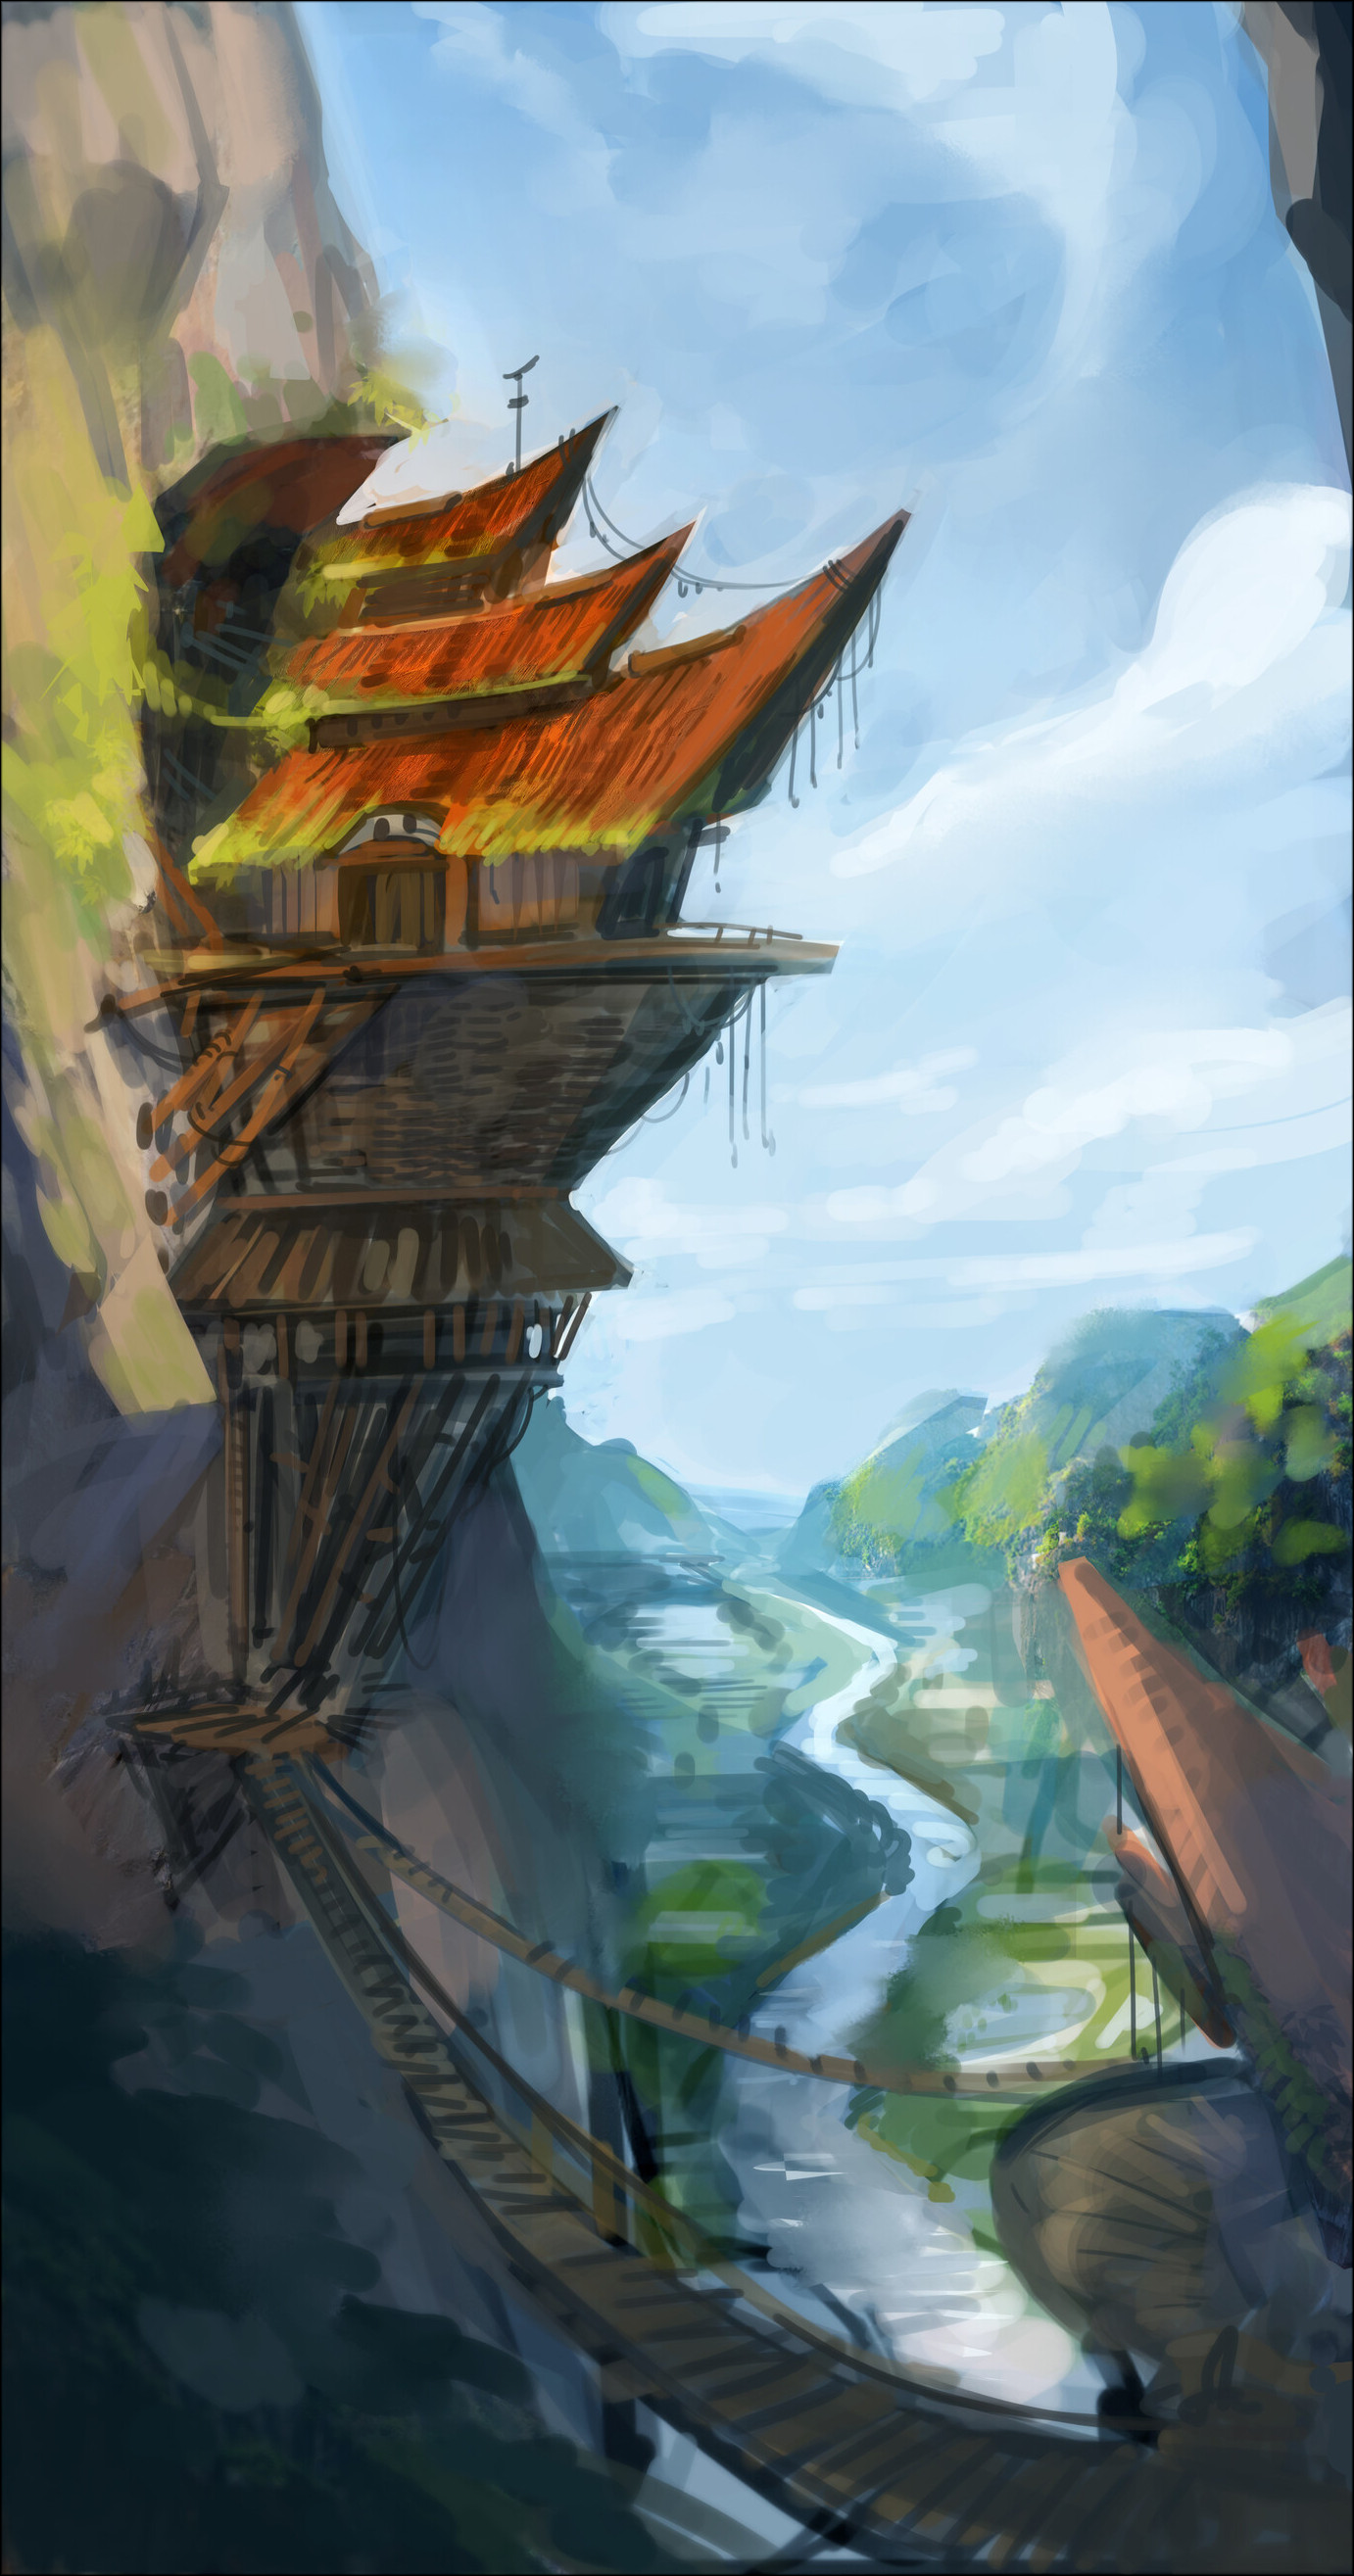
\includegraphics[width=0.46\textwidth]{01yuadrem/img/13siszgoel.png}
    \caption*{\centering \large{\textbf{Siszgoel, Kaldrathal's Capital}}} % TODO: Check if I can change the font of the caption
\end{figure}

\subsection*{Whaler's Sea} \label{ssec::whalerssea}

% intro
The cradle of modern civilization, the Whaler's Sea is home to both well-established and blooming countries.
Its coasts protected from harsh winds by mountain ranges and its cold waters supplied with both whale and idzel, the region couldn't be a better location to develop the modern world.
Idzels are large whale-like creatures known for their ship-sinking fury and their large supply of the valuable ambergris, the main ingredient in artificial qualars.

% Krejek and Kaljek
Sitting at the middle of the sea are the two southernmost islands of the Arctic Archipelago, Krejek and Kaljek.
The first is a large island covered by mountains, rocks plains, and deciduous forests.
It serves as the mainland for the independent nation of Kaldrathal.
%, who competes with Sulia as the main exporter of nitrate.

Starting out as a Krudzalian colony, they merged the quench-hardened steel of the thul'kraka irds with their natural supply of nitrate.
This combination produces resilient steel firearms, including cannons, muskets, and flintlock handguns.
They remain the only exporter of these valuable weapons.

Kaljek, the smaller of the two islands, is a desolate land, with only few pine and birch forests.
It is separated by four nations inhabited by gat and ird alike.
While historically peaceful towards each other, they have recently been divided by conflict, all over the recently discovered gold veins that hide under their land.
% 661 AS: gold veins found under the ground.

% southern coast
South of both islands are the Horned Shores and the Fesh Peninsula.
The first is known for its calm, dry mediterranean climate, its sparse forests, and the great concrete gat city-states that rise from its ground.
Most of the land is devoid of natural resources, with scarce mines and low-quality wood.

% eastern coasts
East to these lands is the Fesh peninsula, an area inhabited mainly by gats, tortles and thul'kraka irds.
A humid subtropical climate permeates the cape, and it is known for its harsh, capricious waters and frequent storms.
Also well-known are the tortles inhabiting the small island of Mbeat, for it is the only place where they have met safety after their arrival in Yuadrem.

In both regions lie the oldest nations of Yuadrem, the Seven kingdoms of the Sea.
Historically renowned raiders and pillagers, they are now famous for their passivity --- focusing on enterprise and artisanship.
What they offer is their expert craftgatship, and among them are the only bonecarvers capable of manufacturing qualars.

% western coast
Finally, to the west of Krejek one can find the two daughters of Palegna, the countries of Sulia and Drer.
The two nations were in a sense ``commisioned'' by the oth nation of Palegna.
Sulia was born to control the worrying growth of the Sulfur Lake, and Drer to restrict the growth of the bughna gat tribes of the Blank Fields.
% Both countries also served as an experiment of sorts for the word-obsessed oths, since the official language in both nations is the artificial Standard Language created by them.

Sulia benefited greatly from what would originally be their burden, and have developed a refined industry based on sulfur.
Their sulfur-based fertilizer is the basis of modern agriculture, their fiery blackpowder is only matched by Kaldrathal's, and their self-preserving wines are a taste craved all around the continent.
% They also have great sulfur-inlaid furniture!

Drer, in stark contrast with its sister, is a nation whose economy solely depends on pillage.
Re-imagining Sulia's blackpowder, they use their fire-bearing weapons to push back and raid their northern neighbors.
